\begin{frame}{Diagnostician}
    \centering
    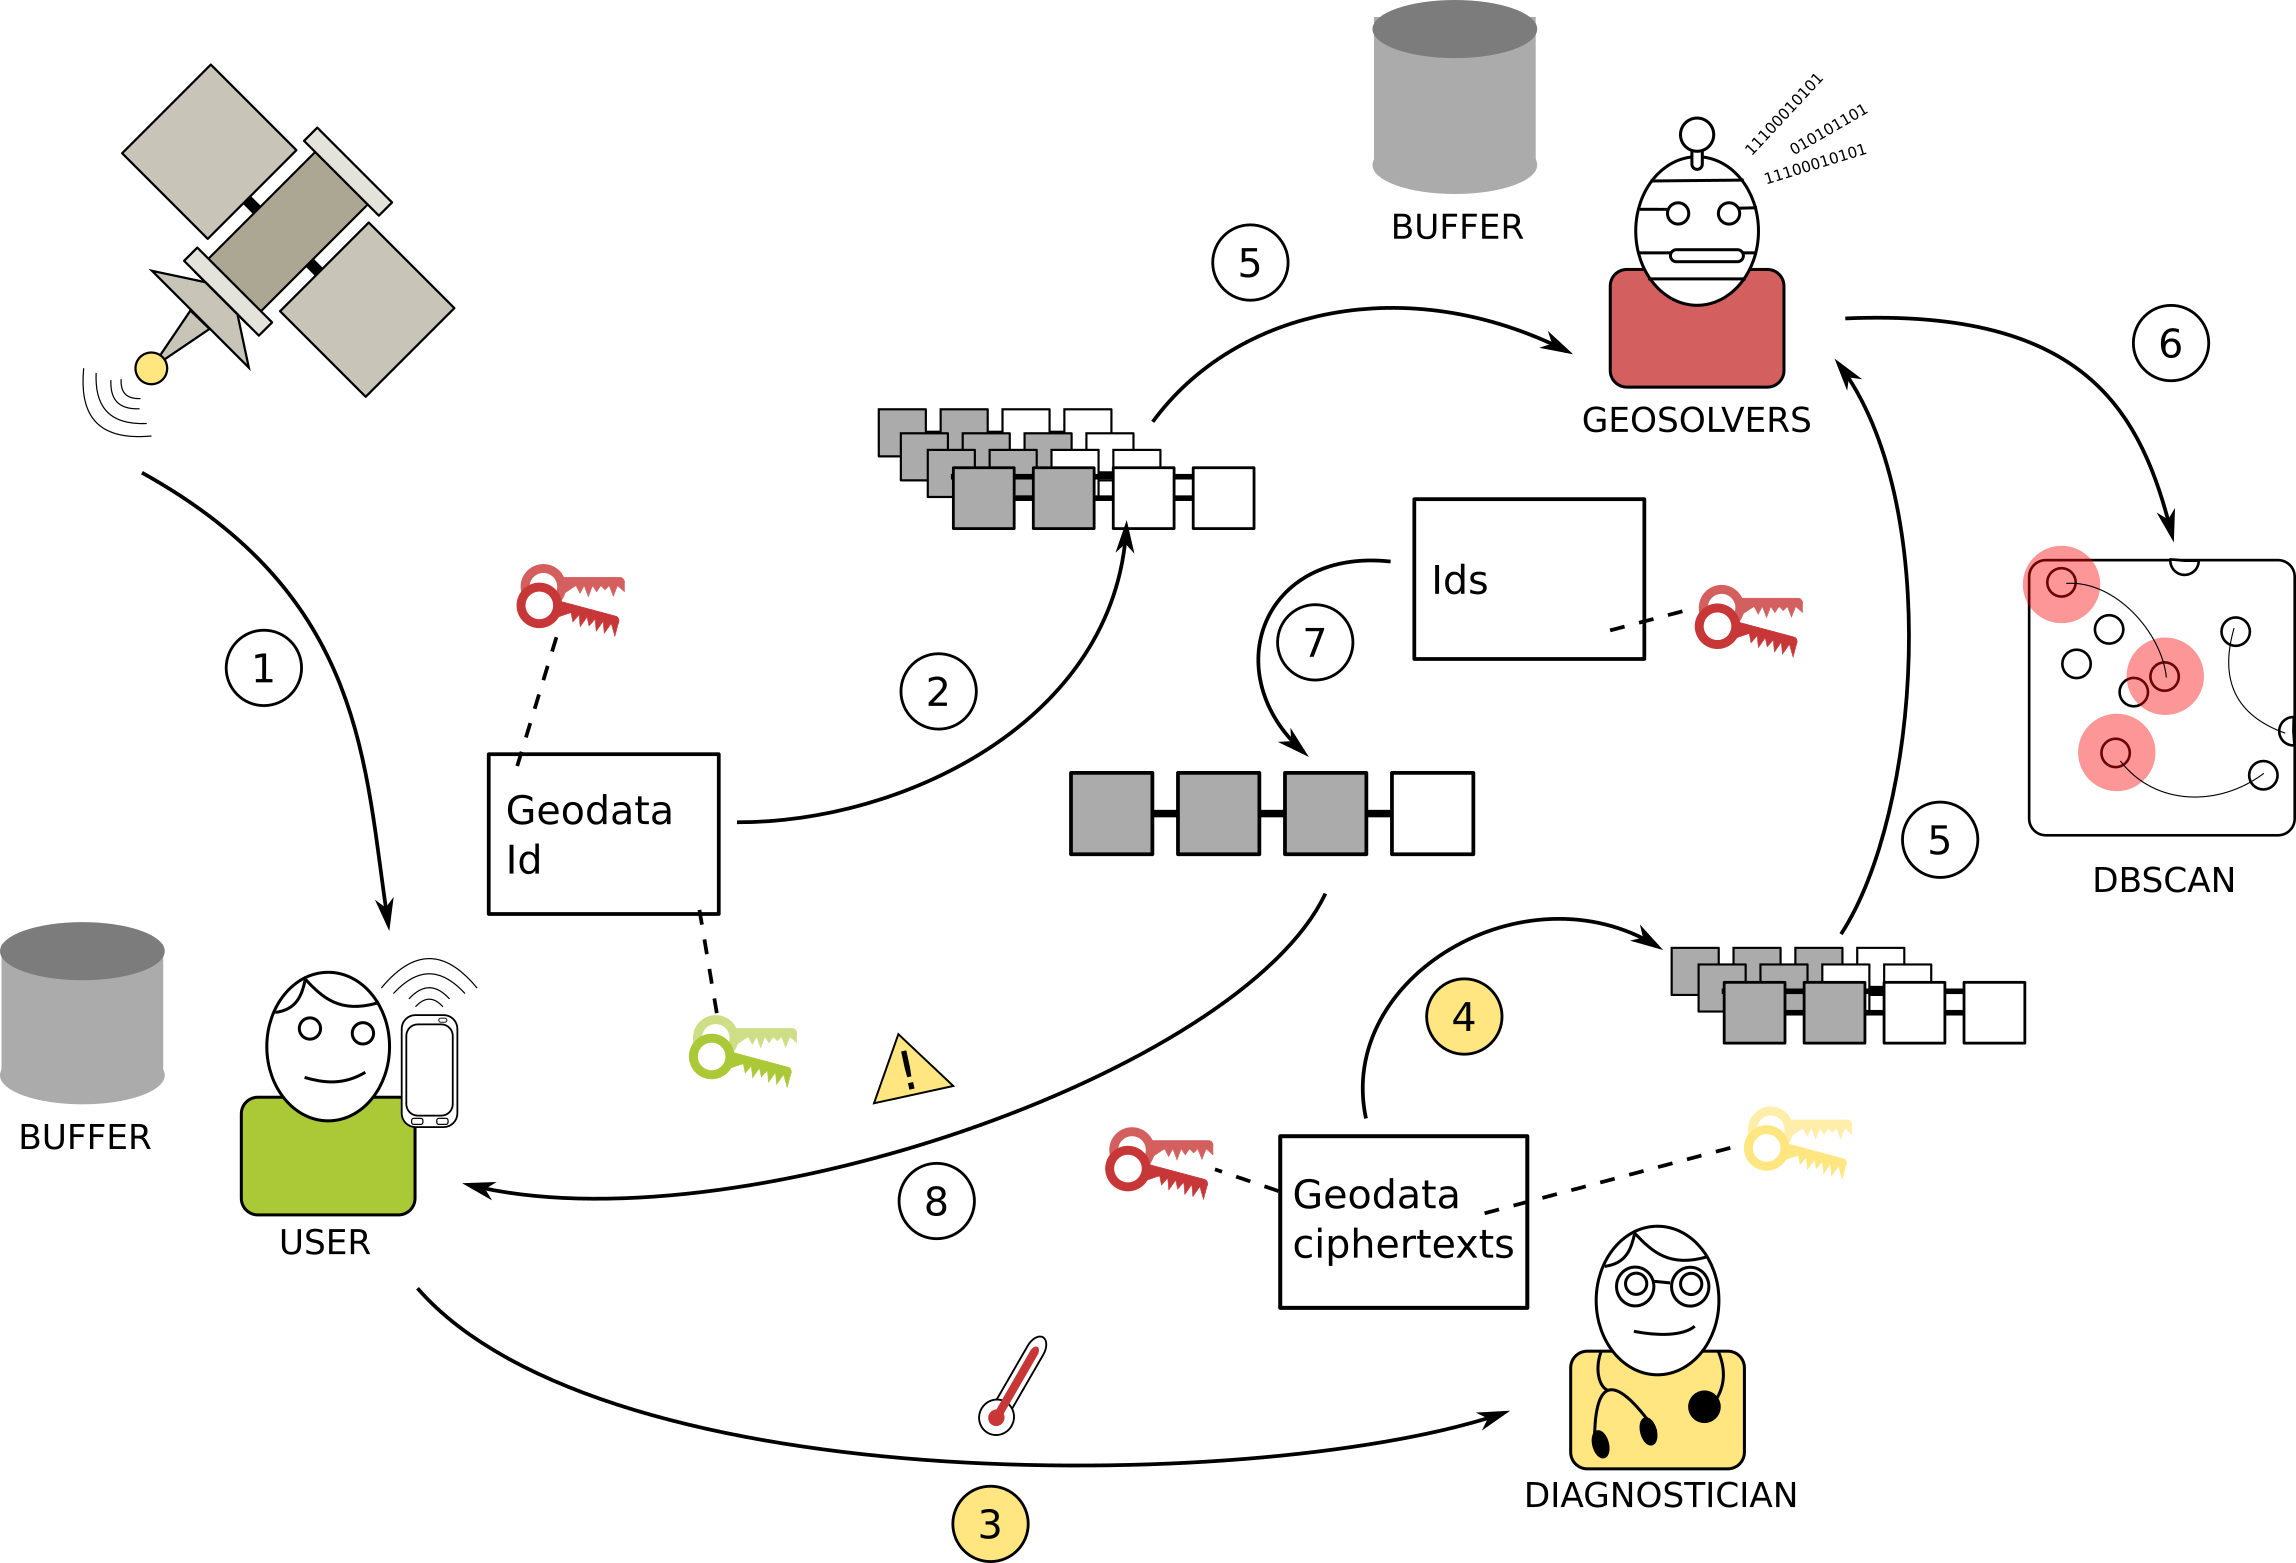
\includegraphics[width=0.95\linewidth]{images/design_diagnosticians.png}
\end{frame}

\begin{frame}{Diagnostician}
    \begin{block}{Characteristics}
        \begin{itemize}
            \item \textbf{GPs} who are in charge to certify positive agents by publishing and signing their data
            \item Own their personal \textbf{MAM channel}
            \item Own a pair of \textbf{keys} to encrypt data for the geosolver
        \end{itemize}
    \end{block}
    
    \vspace{-3pt}
    
    \begin{block}{Certification Procedure}
        Diagnosticians read data from a positive agent's MAM channel, then they:
        \begin{itemize}
            \item [1.] Verify the correctness of the agent's transactions
            \item [2.] Discard the agent's ID from each transaction, so that the geosolver will not know who is the infected agent
            \item [3.] Collect the ciphertext of each transaction, then put them in a list which is paired with the agent's public key so that the geosolver would be able to decrypt it
            \item [4.] Encrypt this pair of data with their private key and the geosolver's public key
            \item [5.] Sign the obtained ciphertext with their private key
            \item [6.] Append the ciphertext to their personal MAM channel, along with the signature and their public key
        \end{itemize}
    \end{block}
\end{frame}